% !TEX root = collection.tex




\section{Computational Indistinguishability}

What should it mean for a computationally bounded adversary to be able to distinguish two distributions from each other? It is tricky to define for a single pair of distributions because the length of the output of a random variable is a constant. Therefore, in order for ``computationally bounded'' adversaries to make sense, we have to work with infinite families of probability distributions.

\begin{definition}
An \emph{ensemble} of probability distributions is a sequence of random variables $\{X_n\}_{n\in \mathbb{N}}$. Two ensembles of probability distributions $\{X_n\}_n$ and $\{Y_n\}_n$ (which are samplable in time polynomial in $n$) are said to be \emph{computationally indistinguishable} if for all (non-uniform) PPT machines $\ma$, the quantities
$$p(n) := \Pr[\ma(1^n, X_n) = 1] = \sum_x \Pr[X_n = x]\Pr[\ma(1^n,x) = 1]$$
and
$$q(n) := \Pr[\ma(1^n,Y_n) = 1] = \sum_y \Pr[Y_n = y]\Pr[\ma(1^n,y) = 1]$$
differ by a negligible amount; i.e. $|p(n) - q(n)|$ is negligible in $n$.    
This equivalence is denoted by
$$\{X_n\}_n\approx \{Y_n\}_n$$
\end{definition}
We now prove some properties of computationally indistinguishable ensembles that will be useful later on.

\begin{lemma}[Sunglass Lemma]
If $\{X_n\}_n\approx\{Y_n\}_n$ and $P$ is a PPT machine, then

$$\{P(X_n)\}_n\approx \{P(Y_n)\}_n$$
\end{lemma}

\proof
Consider an adversary $\ma$ that can distinguish $\{P(X_n)\}_n$ from $\{P(Y_n)\}_n$ with non-negligible probability. Then the adversary $\ma\circ P$ can distinguish $\{X_n\}_n$ from $\{Y_n\}_n$ with the same non-negligible probability. Since $P$ and $\ma$ are both PPT machines, the composition is also a PPT machine. This proves the contrapositive of the lemma.
\qed


\begin{lemma}[Hybrid Argument]
For a polynomial $t:\mathbb{Z}^+\rightarrow\mathbb{Z}^+$ let the $t$-product of $\{Z_n\}_n$ be

$$\{Z_n^{(1)}, Z_n^{(2)},\hdots, Z_n^{(t(n))}\}_n$$
where the $Z_n^{(i)}$s are independent copies of $Z_n$. If
$$\{X_n\}_n\approx\{Y_n\}_n$$
then
$$\{X_n^{(1)},\hdots,X_n^{(t)}\}_n\approx\{Y_n^{(1)},\hdots,Y_n^{(t)}\}_n$$
as well.
\end{lemma}

\begin{proof}
Consider the set of tuple random variables
$$H^{(i,t)}_n = (Y_n^{(1)},\hdots,Y_n^{(i)},X_n^{(i+1)},X_n^{(i+2)},\hdots,X_n^{(t)})$$
for integers $0\le i\le t$. Assume, for the sake of contradiction, that there is a PPT adversary $\ma$ that can distinguish between $\{H^{(0,t)}_n\}_n$ and $\{H^{(t,t)}_n\}_n$ with non-negligible probability difference $r(n)$. Suppose that $\ma$ returns 1 with probability $\epsilon_i$ when it runs on samples from $H^{(i,t)}_n$. By definition, $|\epsilon_t - \epsilon_0|\ge r(n)$. By the Triangle Inequality and the Pigeonhole Principle, there is some index $k$ for which
$|\epsilon_{k+1} - \epsilon_k|\ge r(n)/t$. However, using Sunglass Lemma, note that the computational indistinguishability of $X_n$ and $Y_n$ implies that $\{H^{(k,t)}_n\}_n$ and $\{H^{(k+1,t)}_n\}_n$ are computationally indistinguishable. This is a contradiction. 
\qed
%This is equivalent to trying to distinguish the ensembles $\{(X_n,T_n)\}_n$ from $\{(Y_n,T_n)\}_n$, where $T_n$ is independent of $X_n$ and $Y_n$ ($T_n$ is the random variable representing all coordinates but the $k$-th coordinate). Note that
%
%\begin{align*}
%r(n)/t&\le |Pr[A(Y_n,T_n) = 1] - Pr[A(X_n,T_n) = 1]|\\
%&= |\sum_{x,t} (Pr[Y_n = x,T_n = t] - Pr[X_n = x,T_n = t])Pr[A(x,t) = 1]|\\
%&= |\sum_t Pr[T_n = t]\sum_x (Pr[Y_n = x] - Pr[X_n = x])Pr[A(x,t) = 1]|\\
%&\le \sum_t Pr[T_n = t]\sum_x |Pr[Y_n = x] - Pr[X_n = x]|Pr[A(x,t) = 1]\\
%\end{align*}
%
%so by the probabilistic method there is a $t_0$ for which $r(n)/t\le \sum_x |Pr[Y_n = x] - Pr[X_n = x]|Pr[A(x,t_0) = 1]$. This means that $X_n$ can be distinguished from $Y_n$ with probability difference $r(n)/t$, which is non-negligible (a contradiction).
\end{proof}

\section{Pseudorandom Generators}
Now, we can define pseudorandom generators, which intuitively generates a polynomial number of bits that are indistinguishable from being uniformly random:
\begin{definition}
A function $G:\{0,1\}^n\rightarrow \{0,1\}^{n+m}$ with $m = poly(n)$ is called a \emph{pseudorandom generator} if
\begin{itemize}
\item $G$ is computable in polynomial time.
\item $U_{n+m}\approx G(U_n)$, where $U_k$ denotes the uniform distribution on $\{0,1\}^k$.
\end{itemize}
\end{definition}


\begin{comment}
\begin{theorem}
Consider $F:\{0,1\}^n\rightarrow \{0,1\}^{n+1}$. Construct a function $G:\{0,1\}^n\rightarrow \{0,1\}^{n+m}$ as follows. Let $T:\{0,1\}^{n+1}\rightarrow \{0,1\}^n$ be the function that truncates a string of length $n + 1$ down to its first $n$ digits. Let $S:\{0,1\}^{n+1}\rightarrow \{0,1\}$ be the function that outputs the last bit in a string of length $n + 1$.

Now, let $G$ be the function for which $G(x)_i = (S\circ(F\circ T)^{i-1}\circ F)(x)$ for $i\in m$ and $G(x)_{m+j} = (T\circ (F\circ T)^{m-1}\circ F)(x)_j$ for all $j\in n$.

\begin{figure}[H]
\caption{The construction of $G$. The output of $G$ is the $m + n$ bit vector depicted as a rectangular column with a red border.}
\begin{center}
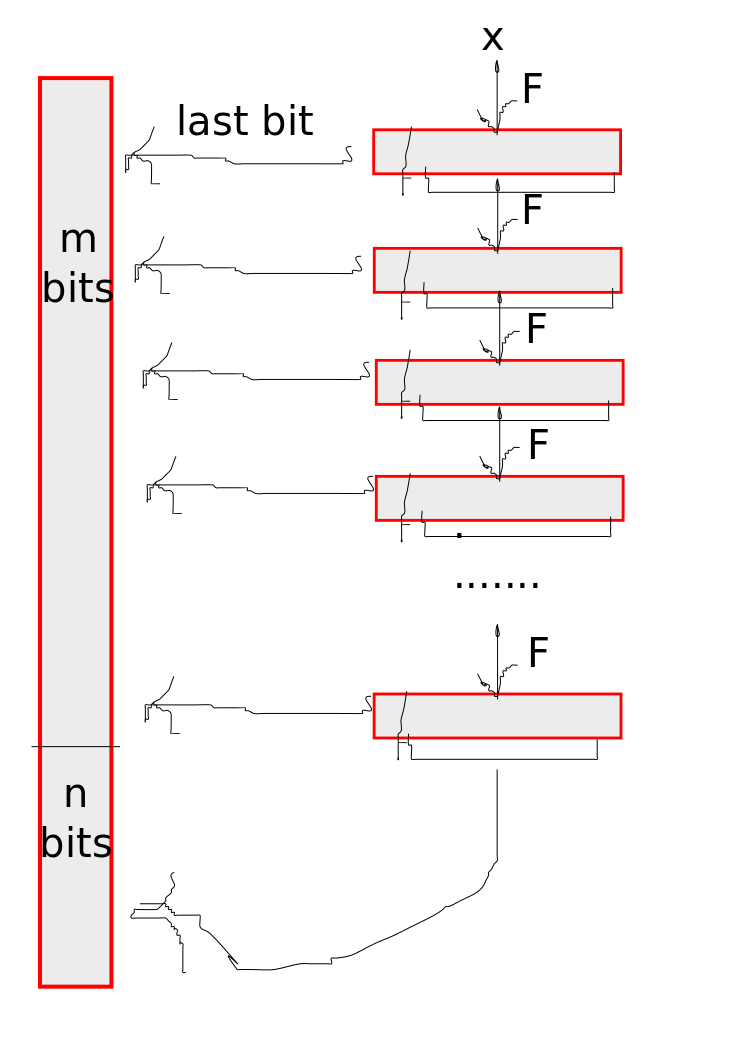
\includegraphics[scale = .3]{prg_strengthening.png}
\end{center}
\end{figure}

$G$ is a pseuodorandom generator if $F$ is also a pseudorandom generator.
\end{theorem}

\begin{proof}
Let $H_i:\{0,1\}^n\rightarrow \{0,1\}^{n+m}$, $0\le i\le m$ be the function that replaces the input to the $i + 1$th function call with $U_n$ and populates the first $i$ bits of the output with $U_i$. Note that $H_0(U_n) = G(U_n)$ and that $H_m(U_n) = U_n$.

Suppose, for the sake of contradiction, that there is a PPT machine $A$ that distinguishes $H_0(U_n)$ from $H_m(U_n)$ with non-negligible probability difference $r(n)$. Then, there is some index $k$ for which $|Pr[A(H_k(U_n)) = 1] - Pr[A(H_{k-1}(U_n)) = 1]|\ge r(n)/m$ by the Pidgeonhole Principle and the Triangle Inequality. These functions can only differ on one bit, though. In particular, the must differ in distribution only on the last bit of the output of the $k$th call to $F$. In particular, $A$ must distinguish $F(U_n)$ from $U_n$ with probability difference at least $r(n)/m$ (since these are the two different inputs to the $k + 1$th call to $f$. $r(n)/m$ is non-negligible, which is a contradiction.
\end{proof}
\end{comment}